\documentclass[12pt]{article}
% REVISION NOTES %%%%%%%%%%%%%%%%%%%%%%%%%%%%%%%%%%%%%%%%%%%%
% 2008-0814 Location, Date, Time
% 2008-0814 fixed citations -- added bibliography.
%
%
\usepackage{geometry}                
\geometry{letterpaper}                   
%\geometry{landscape}                
\usepackage[parfill]{parskip}    
\usepackage{daves,fancyhdr,natbib,graphicx,dcolumn,amsmath,lastpage,url}
\usepackage{amsmath,amssymb,epstopdf,longtable}
\usepackage{enumerate}
\usepackage[final]{pdfpages}
\DeclareGraphicsRule{.tif}{png}{.png}{`convert #1 `dirname #1`/`basename #1 .tif`.png}
\pagestyle{fancy}
\lhead{CE 3305 -- Fluid Mechanics -- SPRING 2024}
\rhead{Name:\_\_\_\_\_\_\_\_\_\_\_\_\_\_\_\_\_\_\_\_\_\_\_\_\_\_\_\_\_\_\_\_\_\_\_\_\_\_\_\_\_\_\_\_}
\lfoot{CE 3305 -- Cleveland}
\cfoot{Page \thepage\ of \pageref{LastPage}}
\rfoot{REVISED: ~1 MAY 2024}
\renewcommand\headrulewidth{0pt}
%%%%%%%%%%%%%%%%%%%%%%%%%%%%%%%%%%%%%%%%%%%%%%%%%%%%%%%
\begin{document}
\section*{\center{ { CE 3305 -- Fluid Mechanics} {Exam 4} } }
\section*{Purpose}
Demonstrate ability to apply fluid mechanics and \textbf{problem solving principles} covering topics such as: Conservation of mass, continunity, conservation of linear momentum, and conservation of energy (modified bernoulli).
\section*{Instructions}
\begin{enumerate}
\item Put your name on each sheet you submit.  
\item Use additional sheets as needed. 
\item Begin each problem on a separate page.  Ok to disassemble to keep pages in order.
\item Do not write on the back of sheets (I won't look)
\item Use the \textbf{problem solving protocol} in the class notes.  The discussion section can simply be the word ``discussion'' 
\item Label and/or underline answers, be sure to include units.
\end{enumerate}
\section*{Allowed Resources}
\begin{enumerate}
\item Your notes
\item Your textbook
\item The mighty Internet with following proviso
\item  \textbf{You may not communicate with other people during the exam}
\end{enumerate}
\noindent\rule{\linewidth}{0.4pt}
\clearpage

\begin{enumerate}
\item The viscosity of a gas increases with increased temperature because

\begin{enumerate}[A)]
\item internal stickiness of the gas decreases.
\item internal molecular activity decreasess.
\item internal stickiness of the gas increases.
\item internal molecular activity increases.
\end{enumerate}

%For gases, viscosity is due to collision between gas molecules. With increase in temperature, gas molecules attain more kinetic energy and the rate of collision is more. Hence, viscosity of gases increases with increase in temperature.

\item Find the difference in pressure between the water and oil if H = 25 cm. 

\begin{figure}[htbp] %  figure placement: here, top, bottom, or page
   \centering
   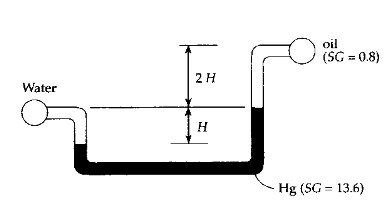
\includegraphics[width=3in]{manometer.png} 
   \caption{}
   \label{fig:manometer}
\end{figure}

\begin{enumerate}[A)]
\item 42.3 kPa
\item 37.2 kPa
\item 34.8 kPa
\item 30.6 kPa
\end{enumerate}

\item The pressure drop across a valve, through which 0.04 $m^3$/s of water flows, is measured to be 100 kPa. Estimate the loss coefficient if the nominal diameter of the valve is 8 cm.
\begin{enumerate}[A)]
\item 0.32
\item 0.79
\item 3.2
\item 8.7
\end{enumerate}
\clearpage


\item Find the expression for the force P needed to hold the gate of width w in the position shown.

\begin{figure}[htbp] %  figure placement: here, top, bottom, or page
   \centering
   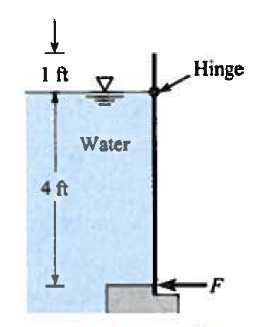
\includegraphics[width=3in]{gate.png} 
   \caption{}
   \label{fig:gate}
\end{figure}

\begin{enumerate}[A)]
\item $\frac{5}{18}\gamma w H^2$
\item $\frac{1}{6} \gamma w H^2$
\item $\frac{2}{9} \gamma w H^2$
\item $\frac{1}{2} \gamma w H^2$
\end{enumerate}

\item The pressure drop over 15 m of 2-cm-diameter galvanized iron pipe is measured
to be 60 kPa. If the pipe is horizontal, estimate the flow rate of water. ($\nu = 10^{-6}
m^2/s$)
\begin{enumerate}[A)]
\item 6.82 L/s
\item 2.18 L/s
\item 0.682 L/s
\item 0.218 L/s
\end{enumerate}

\item Water flows in a pipe of diameter D with a velocity V. It enters at the center of
two parallel disks of radius R separated by a distance t. The water flows radially
outward between the disks. The velocity with which the water leaves the disks is

\begin{enumerate}[A)]
\item $\frac{D^2V}{4R^2}$
\item $\frac{D^2V}{8Rt}$
\item $\frac{DtV}{8R^2}$
\item $\frac{DtV}{4R^2}$
\end{enumerate}

\item What is the energy requirement of an 85\% efficient pump that transports 0.04
$m^3$/s of water if it increases the pressure from 200 kPa to 1200 kPa?
\begin{enumerate}[A)]
\item 4.8 kW
\item 14.2 kW
\item 34.0 kW
\item 47.1 kW
\end{enumerate}

\item Water flows through a converging fitting shown and discharges to the atmosphere as a free jet.
Flow is incompressible, friction negligible.

\begin{figure}[htbp] %  figure placement: here, top, bottom, or page
   \centering
   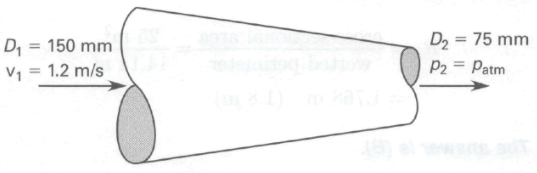
\includegraphics[width=3in]{nozzle.png} 
   \caption{}
   \label{fig:nozzle}
\end{figure}

The gage pressure at the inlet is
\begin{enumerate}[A)]
\item 10.2 kPa
\item 10.8 kPa
\item 11.3 kPa
\item 12.7 kPa
\end{enumerate}

\item A model of a dam is constrycted so the scale of prototype to model is 15:1.  The similarity scaling is based on Froude numbers.  At a certain point on the spillway of the model, the velocity is measured as 5 meters per second. At the corresponding point on the spillway of the actual (prototype) dam, the velocity is about

\begin{enumerate}[A)]
\item 6.7 $\frac{m}{s}$
\item 7.5 $\frac{m}{s}$
\item 15 $\frac{m}{s}$
\item 19 $\frac{m}{s}$
\end{enumerate}

\clearpage

\item 
The canal shown below is to be widened so that the water flow discharge can be tripled (i.e., flow discharge after widening is three times the initial flow discharge). 

\begin{figure}[htbp] %  figure placement: here, top, bottom, or page
   \centering
   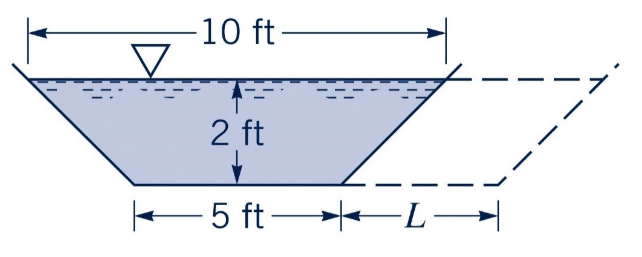
\includegraphics[width=3in]{trapezoid.png} 
   \caption{}
   \label{fig:continunity}
\end{figure}

Determine:
\begin{enumerate}
\item The additional width, $L$, required if all other parameters (i.e., flow depth, bottom slope, surface material, side slope) are to remain the same
\end{enumerate}
%\noindent\rule{\linewidth}{0.4pt}
%\clearpage
%~\newline
%\clearpage
%\item A fixed mass of water has a bulk modulus of compressibility of $2.2 \times 10^{9} ~Pa$. \\ \\
%Determine:
%\begin{enumerate}
%\item The pressure increase ($\Delta p$) required to reduce the volume of a mass of water by 2-percent (2 \%)
%\end{enumerate}
%\noindent\rule{\linewidth}{0.4pt}
%\clearpage
%\noindent\rule{\linewidth}{0.4pt}
\item The figure below is a schematic of water flowing under a sluice gate in a horizontal channel 5 feet wide.

\begin{figure}[htbp] %  figure placement: here, top, bottom, or page
   \centering
   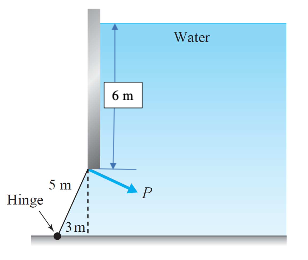
\includegraphics[width=3in]{sluicegate.png} 
   \caption{}
   \label{fig:venturiflow}
\end{figure}

Determine:
\begin{enumerate}
\item Discharge through the sluice gate
\item Power dissipated in the jump
\item The alternate depth (depth of flow after the jump)
\end{enumerate}
%\noindent\rule{\linewidth}{0.4pt}
\clearpage
\item A simple centrifugal pump consists of a 10-cm disk with radial ports shown.  Water is pumped from the reservoir through a central tube coincident with the rotating axis.  The disk rotates at 3000 rpm and discharges to atmospheric pressure.  

\begin{figure}[htbp] %  figure placement: here, top, bottom, or page
   \centering
   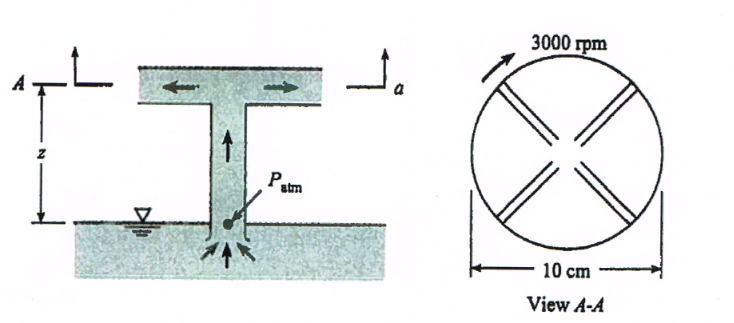
\includegraphics[width=4in]{centrifugepump.png} 
   \caption{}
   \label{fig:centrifugepump}
\end{figure}

Determine:
\begin{enumerate}
\item Shutoff height $z$ for the pump.\footnote{At shutoff flow is zero}
\end{enumerate}


\item Water flows at a steady rate of 192 $\frac{ft^3}{s}$ through a concrete-lined rectangular channel 16 ft wide as depicted in Figure 1. Water enters the 0.35\% sloped channel ($S_0$ = 0.0035) at location 1 and is flowing at 110\% normal depth ($1.1 \times y_n$). The water exits over a 3-foot tall weir (assume sharp-crest weir) at location 2.

\begin{figure}[htbp] %  figure placement: here, top, bottom, or page
   \centering
   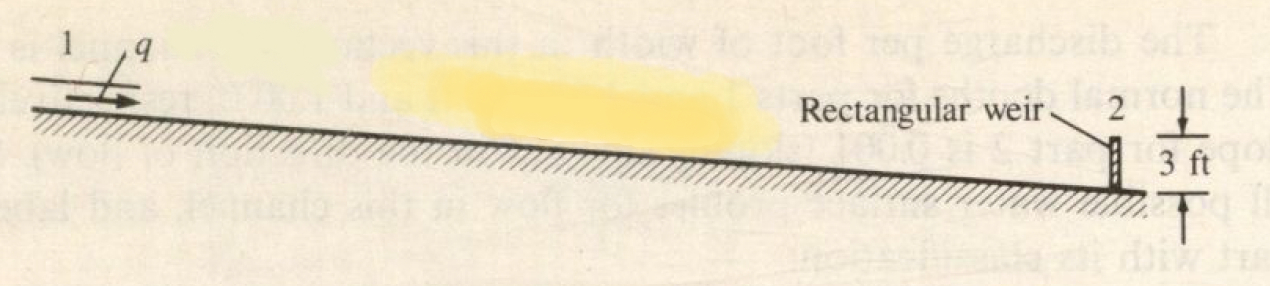
\includegraphics[width=4in]{channel_profile.png} 
   \caption{}
   \label{fig:channel_profile}
\end{figure}

Determine
\begin{enumerate}
\item Normal depth for the channel.
\item Critical depth for the channel.
\item Pool depth just upstream of the weir. (Hint: Add the critical depth to the weir height as an approximation to the pool depth)
\item An estimate of the distance upstream from the weir to location 1 
\end{enumerate}
\clearpage

%~\newline
%\item A small spherical drop of water with diameter $d=4~mm$  and surface tension ($\sigma = 72.8 \times 10^{-3} \frac{N}{m}$) is depicted in the drawing below.

%\begin{figure}[h!] %  figure placement: here, top, bottom, or page
%   \centering
%   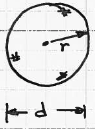
\includegraphics[width=1in]{drop.png} 
%   \caption{}
%   \label{fig:drop}
%\end{figure}

%Determine:
%\begin{enumerate}
%\item The gage pressure of the water in the drop.
%\end{enumerate}
%\noindent\rule{\linewidth}{0.4pt}
%\clearpage
%\noindent\rule{\linewidth}{0.4pt}
%~\newline



\end{enumerate}
%%%%%%%%%%%%%%%%%%%%%%%%%%%%%%%%%%%%%%%%%%%%%%%%%%%%%%%%%%%%%%%%%%%%%%%%%%%%%%%%%%%%
\bibliographystyle{chicago}	         % (uses file "chicago.bst")
\end{document}

\item A windmill is connected directly to a mechanical pump (inertia-type) to lift water from a well that is 10 feet deep as depicted on Figure 5.  The wind turbine is a conventional horizontal-axis type with a fan diameter of 10 feet.  The efficiency of the mechanical pump is 80\%. The pump discharges to atmospheric pressure as shown through 20 feet of 2-inch galvanized pipe.

\begin{figure}[htbp] %  figure placement: here, top, bottom, or page
   \centering
   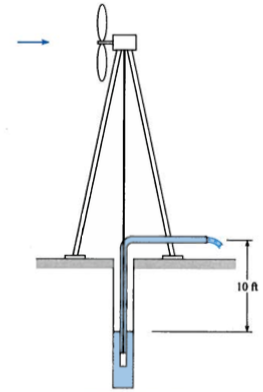
\includegraphics[width=2in]{windmill.png} 
   \caption{}
   \label{fig:windmill}
\end{figure}

For an air density $\rho_{air}=0.07~\frac{lbm}{ft^3}$ and a wind speed of 30 miles per hour

Determine:
\begin{enumerate}
\item Well discharge in gallons per minute 
\end{enumerate}
\clearpage


